\section{Data}\label{data}

The dataset used in this shared task is the IBM Debater(R) - ArgKP v1 \cite{Bar-HaimEFKLS2020} which consists of over 
24.000 argument and key point pairs labeled as matching/non-matching.
They all belong to one of 28 controversial topics ranging from "Assisted suicide should be a criminal offence." to 
"We should abandon marriage." therefore drawing a clear line between supporting and non-supporting key points.

The section used for training has over 5500 arguments belonging to over 200 key points with 24 topics. This leaves the 
dev dataset with over 900 arguments and 36 key points for 4 topics.

\subsection{Characteristics}

\todo{Report data characteristics from exploratory data analysis.}
When analyzing the data, we realize that matched and unmatched key points of a given argument contain a certain proportion of the same words. 
Many of these words belong to the set of stop words. 
These uninformative, non-decisive words can complicate the decision process between the matched and unmatched keypoint. 
For this reason, we remove stop words from our data during pre-processing. 
\begin{figure}[h]
	\label{fig:stopwords-strict}
	\caption{Top 15 most common words of argument keypoint pair for strict labels under the given topic: \texttt{Assisted suicide should be a criminal offence}}
	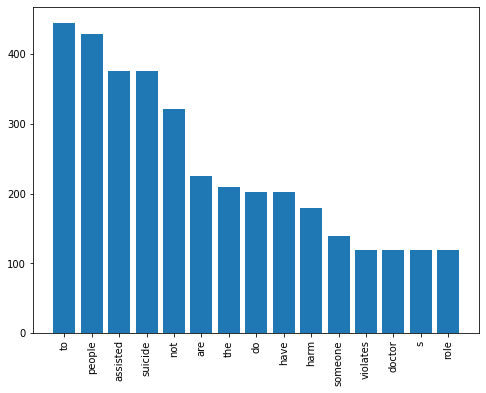
\includegraphics[scale=0.4]{figures/data_stopwords1.png}
\end{figure}
\begin{figure}[h]
	\label{fig:stopwords-relaxed}
	\caption{Top 15 most common words of argument keypoint pair for relaxed labels under the given topic: \texttt{Assisted suicide should be a criminal offence}}
	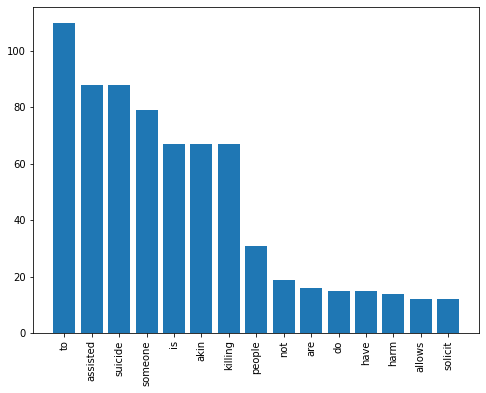
\includegraphics[scale=0.4]{figures/data_stopwords2.png}
\end{figure}
In the figures \ref{fig:stopwords-strict}, \ref{fig:stopwords-relaxed}, we can see that stop words, such as: \texttt{is, are, be, not, to, do, for, have}, are used very frequently in the key points from the two labels. 

Furthermore, the important words from the argument are repeated with different tenses and parts of speech in key points, for example: \textit{legalize, legalized, legalizing, legal} or \textit{marriages, marriage}.
Because these words were used again, they can play a role in classification. 
To achieve an unambiguous spelling, such words are normalized with a stemming method in our approach. 
Moreover, this conversion to the word root reduces the size of the vocabulary or the dimensions of the text input. 
With a low number of dimensions, the assumption of independence of individual features in general machine learning algorithms is violated with a low probability. 

\begin{table*}[]
\caption{Examples of arguments key points from the ArgKP dataset \cite{Bar-HaimEFKLS2020}}
\label{tab:data-example}
\begin{tabular}{l|l|l}
 &
  \textbf{argument} &
  \textbf{key point} \\ \hline
1 &
  \textit{Being a performer harms the child's education} &
  \textit{\begin{tabular}[c]{@{}l@{}}child actors can be overworked and they can \\ miss out on their education\end{tabular}} \\ \hline
2 &
  \textit{\begin{tabular}[c]{@{}l@{}}capital punishment breaks the human rights of \\ the individuals being punished\end{tabular}} &
  \textit{State-sanctioned killing is principally wrong} \\ \hline
3 &
  \textit{\begin{tabular}[c]{@{}l@{}}it is not fair to not allow children to express \\ their personality through dress as long as it\\  is appropriate\end{tabular}} &
  \textit{\begin{tabular}[c]{@{}l@{}}School uniform is harming the student's \\ self-expression\end{tabular}}
\end{tabular}
\end{table*}

In Table \ref{tab:data-example} we show examples of arguments key-point pairs from the ArgKP dataset \cite{Bar-HaimEFKLS2020}. 
We identify followed major difficulties in matching key points to arguments: semantic similar words, synonyms, and context understanding.

In the first example pair (Table \ref{tab:data-example}), the key point can be matched with its argument with a high probability. 
The two sentences were written on the topic of children actors and their education, although the word \texttt{actors} is not explicitly used in the key point. 
We know that \texttt{performer} and \texttt{actors} are semantically relevant and \texttt{performer} and \texttt{actor} both perform. Next, the argument and the key point from the second example were expressed completely differently. 
The important words \texttt{capital punishment}, \texttt{state-sanctioned killing} show us that the two sentences were written at least about the same topic. 
This poses a challenge for us to design our approach in such a way that it knows the different written words with the same meaning. 
A simple method we use is to apply the well-known lexical database WordNet for the English language \cite{Miller1995}.

It is still recognized that context understanding can be a challenge for the task. For this topic from the test dataset:
\texttt{We should abandon the use of school uniform}, we have in the third example an argument and a possible matched key point is \texttt{School uniform is harming the student's self-expression}. 
We can first see that the argument and the given key point have little in common: \texttt{express, expression}. 
To predict if the key point is aligned with the argument, we need to compare their meanings. 
To better deal with the problem of context understanding, we use two well-known language models in our second approach, which we describe in more detail in the next chapter Approach.
